\documentclass{article}

\usepackage{indentfirst}
\usepackage{graphicx}
\usepackage{subfigure}

\begin{document}

\setlength{\parindent}{2em}
\linespread{1}

\title{Project Report : Single Image Haze Removal}
\author{Zeyuan Shang \\ 2011012032 \\ Tsinghua University}
\date{\today}
\maketitle

\section{Introduction}
    
    Images of outdoor scenes are usually degraded by the turbid medium (e.g., particles, water-droplets) in the atmosphere. Haze, fog, and smoke are such phenomena due to atmospheric absorption and scattering. Haze removal1 (or dehazing) is highly desired in both consumer/computational photography and computer vision applications.

    In this project, we experimentally examined approach proposed in \cite{Kaiming}, which could remove haze using single image.

\section{Aproach}

    \subsection{Haze model}

        The model widely used in describing the formation of haze image is as follows:
        
        $$I(x) = J(x)t(x) + A(1 - t(x))$$

        where x is a pixel, I is the observed intensity, J is the scene radiance, A is the global atmospheric light, t is the medium transmission describing the portion of the light that is not scattered and reaches the camera. The goal of haze removal is to recover J, A, and t from I.

    \subsection{Dark Channel Prior}

        Observation shows that, in foggy area of the image, the minimum RGB values of a pixel is higher than that in clear area. An intuition is that, foggy image tends to be “whitish”.

        According to this, we can give an initial estimation of J:

        $$J^{dark}(x) = \min_{c\in\{r, g, b\}} (\min_{y \in \Omega(x)} (J^{c}(y)))$$

        where $J^{c}$ is a color channel of J and $\Omega(x)$ is a local patch centered at x. In \cite{Kaiming}, it is called dark channel prior. A typical size of the patch is 15x15, and $\omega$ is arount 0.95.

        As observation shows, nice property of $J^{dark}$ is that, for a haze free image J, $J^{dark} \to 0$.

    \subsection{Estimate the Atmospheric Light}

        We pick the top 0.1\% brightest pixels in dark channel, and pick the highest intensity in input image I as atmospheric light.

    \subsection{Estimate the Transmission}

        First assume that the atmospheric light A is known, By further assuming the transmission in a local patch $\Omega(x)$ is constant, the property of $J^{dark}$, after crunching equations, we get:

        $$\widetilde{t}(x) = 1 - \min_{c} (\min_{y \in \Omega(x)} (\frac{I^{c}(y)}{A^{c}}))$$

        where $\widetilde{t}(x)$ is the estimation of true transmission $t(x)$. But even in clear days, atmosphere is not absolutely free of any particle, the haze effect may still slightly appears. The catch this observation, an constant parameter $\omega(0 < \omega <= 1)$. The equation above then becomes:

        $$\widetilde{t}(x) = 1 - \omega \min_{c} (\min_{y \in \Omega(x)} (\frac{I^{c}(y)}{A^{c}}))$$


    \subsection{Transmission Refinement}

        In the original paper, the transmission is then refined using soft matting introduced in \cite{Anat}.  Rewriting $t(x)$ and $\widetilde{t}(x)$ in their vector form as $t$ and $\widetilde{t}$, we minimize the following cost function:

        $$E(t) = t^{T} L t + \lambda (t - \bar{t})^{T} (t - \bar{t})$$

        where L is the Matting Laplacian matrix proposed by \cite{Anat}, and $\lambda$ is a regularization parameter.

        The (i,j) element of the matrix L is defined as:

        $$\sum_{k|(i, j) \in w_{k}} (\delta_{ij} - \frac{1}{|w_{k}|} (1 + (I_{i} - \mu_{k})^{T} (\Sigma_{k} + \frac{\epsilon}{|w_{k}|} U_{3})^{-1} (I_{j} - \mu_{k})))$$

        where $I_{i}$ and $I_{j}$ are the colors of the input image I at pixels i and j, $\delta_{ij}$ is the Kronecker delta, $\mu_{k}$ and $\Sigma_{k}$ are the mean and covariance matrix of the colors in window $\omega_{k}$, $U_{3}$ is a 3×3 identity matrix, $\epsilon$ is a regularizing parameter, and $|w_{k}|$ is the number of pixels in the window $\omega_{k}$.

        The optimal t can be obtained by solving the following sparse linear system:

        $$(L + \lambda U) t = \lambda \widetilde{t}$$

        where U is an identity matrix of the same size as L. Here, we set a small value on $\lambda$ ($10^{-4}$ in our experiments) so that t is softly constrained by $\widetilde{t}$.

    \subsection{Recover the Scene Radience}

        From equation aforementioned, it is direct that we can recover $J(x)$ by

        $$J(x) = \frac{I(x) - A}{\max(t(x), t_{0})} + A$$

        where $t_{0}$ is the minimum transmission threshold, typically around 0.1.

\section{Result}

    See figures below.

    \begin{figure}
        \begin{center}
            \subfigure[input]{
                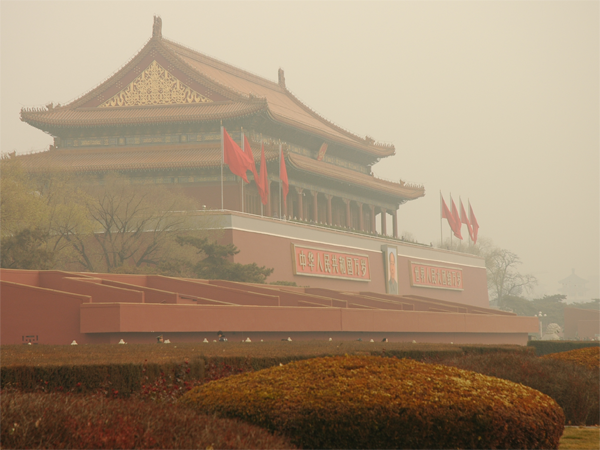
\includegraphics[height=0.3\textheight, width=0.6\textwidth]{tiananmen.png}
            }
            \subfigure[before soft matting]{
                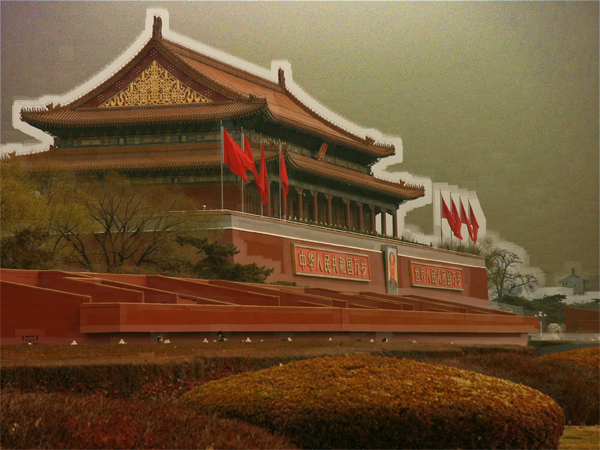
\includegraphics[height=0.3\textheight, width=0.6\textwidth]{semi_tiananmen.png}
            }
            \subfigure[output]{
                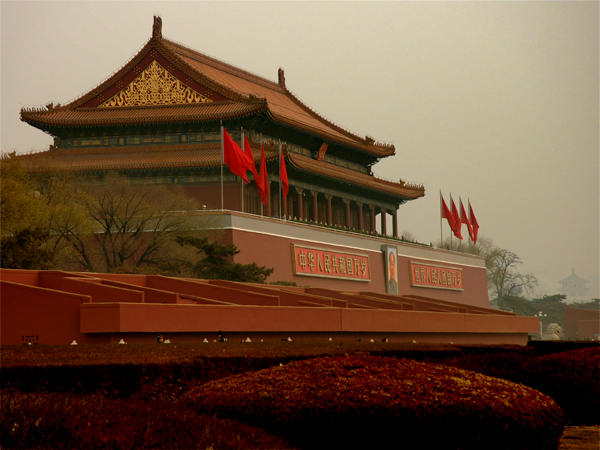
\includegraphics[height=0.3\textheight, width=0.6\textwidth]{output_tiananmen.png}
            }
        \end{center}
        \caption{Tiananmen}
    \end{figure}

    \begin{figure}
        \begin{center}
            \subfigure[input]{
                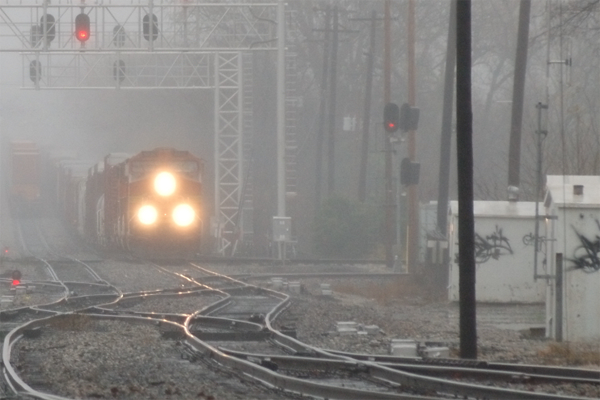
\includegraphics[height=0.3\textheight, width=0.6\textwidth]{train.png}
            }
            \subfigure[before soft matting]{
                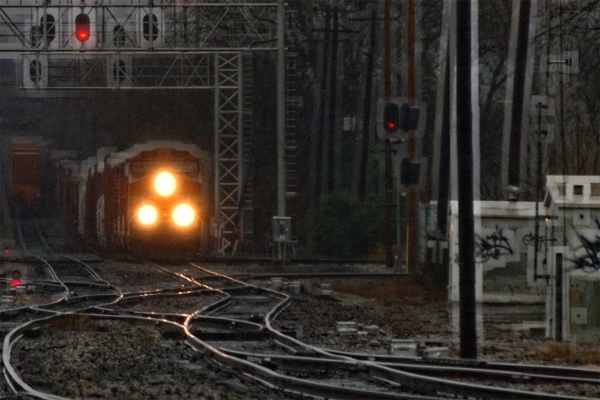
\includegraphics[height=0.3\textheight, width=0.6\textwidth]{semi_train.png}
            }
            \subfigure[output]{
                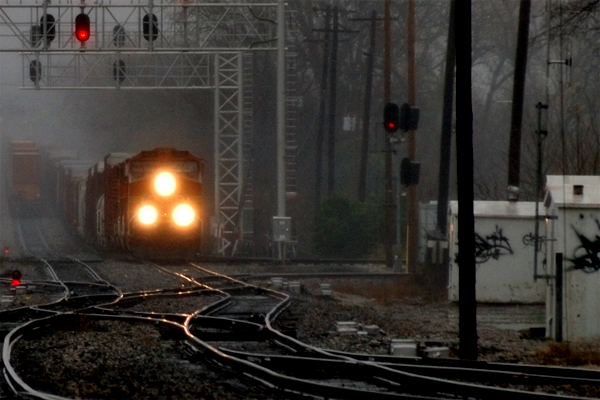
\includegraphics[height=0.3\textheight, width=0.6\textwidth]{output_train.png}
            }
        \end{center}
        \caption{Train}
    \end{figure}

\renewcommand\refname{Reference}
\bibliographystyle{plain}
\bibliography{doc}

\end{document}